% fpga.tex
\chapter{FPGAs}
Die Arbeit befasst sich mit der Implementierung und Optimierung von Logistischer Regression auf FPGAs. Deshalb wird zunächst der allgemeine Aufbau dieser beschrieben. Dann folgt eine Einführung in die Konfiguration des FPGAs, wobei zum einen auf den typischen Ablauf, zum anderen auf die verwendeten Programme eingegangen wird. Abschließend wird die verwendete Hard- und Software aufgeführt.
\section{Allgemeiner Aufbau von FPGAs}
Field Programmable Gate Arrays (FPGAs) sind Integrierte Schaltkreise (IC) in die eine logische Schaltung programmiert werden kann. Die ICs bestehen aus I/O-Blöcken, Programmierbaren Logikblöcken (Configurable Logig Blocks, kurz CLB) und weiteren Bestandteilen wie zum Beispiel DSP-Slices, BRAM-Blöcken, Multipliziereinheiten oder Taktgeneratoren welche durch Datenpfade zu einer Matrix miteinander verbunden sind (Siehe Abbildung 2.1).\\
\begin{figure}[ht]
	\begin{minipage}[b]{.4\linewidth}
  		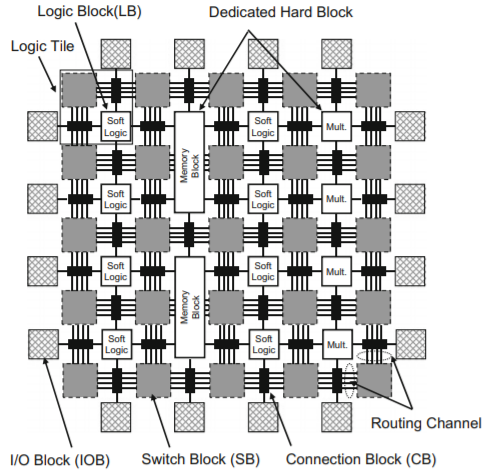
\includegraphics[scale=0.7]{bilder/matrix}
  		\caption{Aufbau eines IC, die grauen Schaltblöcke (SB) sind die konfigurierbaren Datenpfade}
  	\end{minipage}
  	\hspace{.1\linewidth}% Abstand zwischen Bilder
  	\begin{minipage}[b]{.4\linewidth}
  		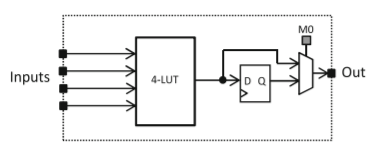
\includegraphics[scale=0.70]{bilder/clp}
		\caption{Schematische Darstellung eines CLB\\
		}
	\end{minipage}
	
\end{figure}
Die Pfade können je nach Bedarf geschaltet werden. Die CLBs selbst bestehen aus einem 1 Bit Flip-Flop und einer programmierbaren Wahrheitstabelle. Über diese lassen sich die logischen Funktionen konfigurieren\cite{TOSU}. Ein schematischer Aufbau ist in Abbildung 2.2 zu sehen. Dieser Aufbau ist typisch für ein FPGA der Marke Xilinx und nicht allgemein für andere Hersteller gültig. Da in dieser Arbeit (wie in Kapitel 2.3 beschrieben) ein FPGA der Marke Xilinx benutzt wird, wird auch dessen Hardwarekonfiguration zugrunde gelegt.\\\\
Die Programmierung ist in diesem Fall vergleichbar mit einer Schalttabelle, welche bestimmt wie die physikalischen Bausteine miteinander verbunden werden sollen. Anders als bei Application-Specific Integrated Circuits
(ASICs), dessen Funktion bereits bei der Produktion festgelegt werden, können FPGAs vom Benutzer selbst Konfiguriert werden. \newpage 
Dies geschieht jedoch im Gegensatz zu Mikroprozessoren nicht während, sondern vor Inbetriebnahme des Chips. Zwar ist es bei
einigen wenigen Herstellern von FPGAs mittlerweile möglich, diese auch wärend des laufenden Betriebs zu konfigurieren (partielle Rekonfiguration), aber das ist mit einer höheren
Komplexität der zu konfigurierenden Logik verbunden.\\
Durch die Konfigurierbarkeit des FPGAs ergeben sich bautechnisch bedingt einige Nachteile gegenüber den ASICs. FPGAs sind annäherungsweise 20 bis 35 mal größer und zwischen 3 und 4 mal langsamer als eine vergleichbare ASIC Implementierung. Außerdem verbrauchen sie dynamisch circa 10 mal mehr Energie \cite{KURO}.
%Vergleich mit CPU und GPU
Damit sind sie deutlich ineffizienter als ASICs. Der große Vorteil ergibt sich hier aus der Konfigurierbarkeit, denn ASICs sind nach der Produktion nicht mehr veränderbar. Besonders in Bereichen die eine hohe Flexibilität verlangen ist es vor allem Kosteneffizienter FPGAs zu benutzen, denn die Produktion von ASICs ist mit großen zeitlichen und finanziellen Investitionen verbunden\cite{KUTERO}.\\
Im Vergleich zu einer CPU ist der Vorteil des FPGA seine hohe Parallelität, denn wo ein handelsüblicher 8-Kern Prozessor nur 8 parallele Aufgaben durchführen kann, da ist die Begrenzung der parallelen Programme auf dem FPGA einzig durch seine Hardwarebausteine begrenzt. Diese Eigenschaft gilt auch für GPUs, welche aber einen so hohen Energieverbrauch haben, dass die in dieser Arbeit nicht behandelt werden. Für GPUs existieren zudem viele Implementierungen von Lernalgorithmen, da man ihren Nutzen dafür bereits erkannt hat.
\section{Konfiguration und Ablauf}
Wie das "`Field Programmable"' im Namen schon besagt ist es möglich nach der Fabrikation des FPGA Funktionen in diese "`in the field"', also im praktischen Einsatz zu programmieren \cite{KUTERO}. Um seine Funktion zu verändern muss das FPGA neu Konfiguriert werden. Dies geschieht durch einen sogenannten "`Bitstream"', eine Sequenz von einzelnen Bits. In Abbildung 2.3 zeigt sich der Ablauf zur Generierung einen solchen Bitstreams für ein FPGA der Marke Xilinx.\\
\begin{figure}[ht]
\begin{tikzpicture}[
    mynode/.style={rectangle,rounded corners,draw=black,
    top color=tugreen!50, bottom color=tugreen!50,thick, inner sep=1em, minimum size=3em,text centered},
    plus/.style={circle,draw=black,
    top color=tugreen, bottom color=tugreen,thick, text centered},
    myarrow/.style={-{Stealth}, shorten >=1pt, thick},
    myarrowdot/.style={-{Stealth}, shorten >=1pt, thick, dashed},
    mydots/.style={dashed, thick},
    line/.style={thick},
    inpnode/.style={},
    dotsred/.style={dashed, thick, color=cred},
    dotsblue/.style={dashed, thick, color=cblue}
]
\node[text width=2cm ,text centered] (dm) {Code in\\ Hochsprache};
\node[mynode, right=1cm of dm, text width=2.2cm](csim){Simulation Hochsprache};
\node[above=1.25cm of dm] (dummydm) {};
\node[mynode, right=1cm of csim, text width=2.2cm](hls){High-Level\\ Synthese};  
\node[mynode, right=1cm of hls, text width=2.2cm](cosim){HS/RTL\\ Kosimulation }; 
\node[mynode, below=2cm of cosim, text width=2.2cm](bd){Blockdesign\\ };
\node[above=1cm of hls] (dummyhls) {};
\node[below=0.8cm of hls] (dummyhlsb){};
\node[right=3.35cm of dummyhlsb](dummycosim){};
\node[mynode, left=1cm of bd, text width=2cm](sim){Simulation};  
\node[mynode, left=1cm of sim, text width=2cm](synth){Synthese};  
\node[mynode, left=1cm of synth, text width=2cm](impl){Implemen- tierung};     
\node[above=1cm of hls](space){};
\node[below=1cm of impl, text width=2.2cm, ,text centered](bs){Fertiger\\ Bitstream};
\node[above=1cm of cosim, text width=2.2cm, ,text centered](rtl){Code in HDL};


\node[left=0.1cm of dm](ring1r){};
\node[above=3cm of ring1r](ring2r){};
\node[right=1cm of ring2r,color=cred](ring2ar){Vivado HLS};
\node[right=11.3cm of ring2ar](ring3r){};
\node[below=5.23cm of ring3r](ring4r){};
\node[below=2cm of ring1r](ring7r){};
\node[above=0.03cm of ring7r](ring1b){};
\node[right=14.6cm of ring1b](ring2b){};
\node[below=4.5cm of ring2b](ring3b){};
\node[below=4.5cm of ring1b](ring4b){};
\node[right=4cm of ring4b, color=cblue](ring5b){Vivado Desing Suite};

\draw[mydots]  (dm.north) -- (dummydm.south);
\draw[mydots]  (dummydm.east) -- (dummyhls.west);
\draw[myarrowdot]  (dummyhls.south) -- (hls.north);
\draw[myarrow] (dm.east) -- (csim.west);
\draw[myarrow] (csim.east) -- (hls.west);
\draw[myarrow] (hls.east) -- (cosim.west);
\draw[myarrow] ($(cosim.south)!0.25!(cosim.south east)$) -- ($(bd.north)!0.25!(bd.north east)$);
\draw[myarrowdot] (dummycosim) -- ($(bd.north)!0.25!(bd.north west)$);
\draw[mydots] (hls.south) -- (dummyhlsb);
\draw[mydots] (dummyhlsb) -- (dummycosim);
\draw[myarrow] (bd.west) -- (sim.east);
\draw[myarrow] (sim.west) -- (synth.east);
\draw[myarrow] (synth.west) -- (impl.east);
\draw[myarrow] (impl.south) -- (bs.north);
\draw[myarrowdot] (rtl.south) -- (cosim.north);
\draw[dotsred] (ring1r) -- (ring2r);
\draw[dotsred] (ring2r) -- (ring2ar);
\draw[dotsred] (ring2ar) -- (ring3r);
\draw[dotsred] (ring3r) -- (ring4r);
\draw[dotsred] (ring4r) -- (ring7r);
\draw[dotsred] (ring7r) -- (ring1r.north);
\draw[dotsblue] (ring1b) -- (ring2b);
\draw[dotsblue] (ring2b) -- (ring3b);
\draw[dotsblue] (ring3b) -- (ring5b);
\draw[dotsblue] (ring5b) -- (ring4b);
\draw[dotsblue] (ring4b) -- (ring1b);
\end{tikzpicture}
\caption{Konfigurationsablauf eines Xilinx-FPGAs}
\end{figure} \\
Historisch bedingt wurde die RTL (Register Transfer Level) für einen Xilinx-FPGA grundsätzlich in einer HDL (Hardware Definition Language) programmiert. Erst seit 2012 gibt es die Tools Vivado Design Suite und Vivado HLS mit denen zusätzlich eine Programmierung in einer Hochsprache, bei Xilinx sind C/C++,  möglich ist. Somit ist diese Möglichkeit noch relativ neu und nicht so weit verbreitet wie die Benutzung von HDLs \cite{XIL4}.
Auch wenn der direkte Ansatz zu effizienteren Designs führen kann ist er doch mit erheblichem Mehraufwand verbunden. Vor allem der geringere Programmieraufwand in C++ gegenüber einem nicht signifikantem Leistungsverlust ist ausschlaggebend dafür, dass dieser Ansatz in der Arbeit nicht weiter behandelt wird, jedoch einen Ausblick auf weitere Verbesserungsmöglichkeiten bietet.\\\\
In dem von Xilinx für die High-Level Synthese vorgesehenem Workflow programmiert man nun zunächst die geplante Anwendung/Funktion in einer beliebigen Hochsprache, zum Beispiel BSV in Bluespec oder MaxJ in MaxCompiler. Die am häufigsten verwendete Sprache ist jedoch C oder C++, wie auch in diesem Fall mit Vivado HLS\cite{NASI}.\\\\ Dann folgt eine Simulation des Programms um dessen Tauglichkeit für eine FPGA Konfiguration zu prüfen. Hierbei wird die Funktionalität des eingegebenen Codes getestet, noch bevor es in die HDL übersetzt wird. Dieser Schritt ist optional, jedoch sehr hilfreich, denn die High-Level Synthese von Vivado HLS nimmt sowohl Zeit als auch Ressourcen auf dem Hostrechner in Anspruch und unterstützt zudem nicht alle Besonderheiten und Datentypen von C++. Es können zum Beispiel keine Arrays mit variabler (zur Laufzeit definierter) Länge instanziiert oder rekursive Funktionen verwendet werden. Außerdem werden Anfragen an das System nicht unterstützt und die Hauptfunktion muss die gesamte Funktionalität des Designs enthalten \cite{XIL2}.\\Nun wird mit der High-Level Synthese ein Programm in einer HDL, in diesem Fall VHDL oder Verilog, erstellt.\\
Man kann nun die Hochsprache und die RTL nebeneinander (ko-) simulieren, um das Verhalten der HLS zu verifizieren. Auch dieser Schritt ist optional und dient der frühen Fehlerfindung. Er führt eine erneute Kontrolle der Funktionalität durch um auszuschließen, dass bei der Übersetzung unerwünschte oder ungeplante Verhaltensweisen auftreten. \\
Nach diesem Schritt wird das RTL-Design als IP (Intellectual Property) exportiert und mit der Vivado Design Suite von Xilinx weiter bearbeitet. Zusammen mit IP-Blöcken von Xillinx und Drittanbietern erstellt man nun ein funktionstüchtiges Design, indem man die Ein- und Ausgänge der Blöcke sinnvoll miteinander verknüpft.\\ Das erstellte Projekt geht jetzt in den Simulaionsschritt, bei dem das echte Verhalten des FPGA emuliert werden soll. Auch diese Simulation überprüft die Funktionalität des Designs, da durch das eventuelle Anfügen weiterer IP Blöcke an das selbst geschriebene Programm und das Verknüpfen der I/O-Schnittstellen mit den simulierten Hardwarekomponenten eines FPGA unbeabsichtigtes Fehlverhalten der Konfiguration auftreten können.\\\\ Im darauffolgenden Syntheseschritt wird durch die Software ein Schaltplan der Funktion erstellt, der die Hardwareprogrammierung auf einem theoretischen FPGA (mit unbegrenzten Hardwarebausteinen) darstellt. Hierbei werden erste Berichte zu der Ressourcenauslastung, dem Timing und dem Energieverbrauch erstellt. Diese sind allerdings nur Schätzungen und dienen dem Auffinden von groben Fehlern, zum Beispiel wenn mehr Ressourcen verbraucht werden würden als das FPGA hat.\\
Im Implementierungsschritt werden nun der vorhandene Netzplan auf das spezifizierte FPGA angewendet und konkrete Vernetzungen errechnet. Die dabei erstellten Berichte sind nun genau, sodass etwaige Fehler nun korrekt behoben werden können. Man kann nun auch einen Schaltplan des FPGA einsehen, in dem alle tatsächlich verwendeten Bausteine markiert sind.
Aus dem implementierten Design kann nun der Bitstream erstellt werden, mit dem der FPGA dann programmiert wird.
\section{Verwendete Hardware}
Das in dieser Arbeit verwendete Board ist ein AC701 Evaluation Kit der Firma Xilinx Inc. Darauf enthalten ist ein FPGA der Serie Artix-7, genauer XC7A200T-2FBG676C. Dieses enthält 215.360 Logikzellen, 740 DSP48E1 (Digital Signal Processor) Slices, 13.140 Kb Block RAM, 33.650 CLB Slices und 500 I/O Pins \cite{XIL3}.
\\Des weiteren sind Auf dem Board unter Anderem 1GB DDR3 RAM Speicher, 256 Mb Flash Speicher, ein SD (Secure Digital) Connector, Mehrere Clock Generatoren (zum Beispiel ein Fixed 200 MHz LVDS oscillator), Status LEDs und konfigurierbare Schalter verbaut.\\
Als Kommunikationsschnittstellen stehen jeweils eine Gen1 4-Lane (x4) und eine Gen2 4-Lane (x4) PCI Express Schnittstelle, ein SFP+ (Enhanced Small Form-factor Pluggable) Connector, ein HDMI (High Definition Multimedia Interface) Ausgang, UART (USB zu Universal Asynchronous Receiver Transmitter) Brücke und eine 10/100/1000 MBit/s tri-speed Ethernet PHY (Physikalische Schnittstelle) zur Verfügung\cite{XIL1}.\\
Eingebaut ist das Board in einen Dektop-PC einem Intel Xeon W3565 Prozessor und 24 GB DDR3 RAM, welcher unter Ubuntu 14.04.5 LTS 64-Bit betrieben wird. Da Board ist über die UART Schnittstelle mit einem USB-Ausgang dieses Rechners verbunden und wird darüber konfiguriert.
Das Erstellen der Software und der Bitstreams erfolg über einen Desktop PC mit einer AMD Phenom$^{TM}$ II X4 960T CPU und 8 GB DDR3 RAM.
\section{Verwendete Software}
Für die High Level Synthese und die Generierung des Bitstreams werden Vivado HLS  und die Vivado Design Suite von Xilinx verwendet. Die Kommunikation mit dem FPGA und dem Host-Rechner erfolgt über PCIe mit einem IP-Core von Xillybus \cite{XILLY}. Die Arbeit baut in dieser Hinsicht auf "`Umsetzung einer High-Performance FPGA-Schnittstelle für maschinelles Lernen"' von Dillkötter\cite{DILL} auf. Die entworfenen Bitstreams werden über den Hardaware-Manager von Xilinx auf das FPGA geladen, sodass mit dem Hostrechner nur über SSH (Secure Shell) gearbeitet wird.